\documentclass [12pt, letterpaper, twoside] {article}
\usepackage[utf8]{inputenc}
\usepackage [left=1.0in, right=1.0in, top=1.0in, bottom=1.0in] {geometry}
% For updated time
\usepackage {datetime}
% For drawing pictures
\usepackage {tikz}
% For equations
\usepackage {amsmath}
% To make tables
\usepackage {tabu}
% For multiple rows in table slot
\usepackage {multirow}
\usepackage {verbatim}
% To add captions
\usepackage {caption}
\usepackage {float}
% To make graphs
\usepackage {pgfplots}
% To make scatter plots
\usepackage{pgfplotstable}

\usetikzlibrary {shapes.geometric, arrows, angles}

\tikzstyle {pink1circle0} = [circle, minimum size=0.5cm, text centered, draw=black, fill=pink1]
\tikzstyle {arrow} = [thick, ->, >=stealth]
\renewcommand {\labelitemiv}{$\triangle$}

\raggedbottom
\begin {document}
\begin {titlepage}
\begin {center}
Department of Biological, Chemical, and Physical Science\\
\vspace {0.1cm}
Illinois Institute of Technology\\
\vspace {0.1cm}
General Physics II: Electromagnetism (PHYS 221-01)\\
\vspace* {\fill}
\begingroup
\Large
\textbf {Electric Fields and Electric Potential}
\vspace {0.35cm}

\normalsize
Lab 3
\vspace {1.5cm}
\endgroup
\vspace* {\fill}
\end {center}

\vspace*{\fill}
\begin {flushright}
\footnotesize
Emily Pang, Lavanya Roy (lab partner) \\
Date of experiment: 12 Feb 2020 \\
Due date: 19 Feb 2020 \\
Lab section L06 \\
TA: Will Limestall \\
Updated \usdate\today~(\currenttime)
\end {flushright}
\end {titlepage}
\subsection* {STATEMENT OF OBJECTIVE}
The objective of this lab was to understand the relationship between field lines and equipotential lines using concepts of electricity, including Coulomb's Law and electric potential. \\

\subsection* {THEORY}


\subsection* {EQUIPMENT}
  \noindent
  \begin {itemize}
    \itemsep0em
    \item {two pith balls}
    \item {one simple electroscope}
    \item {mirror ruler}
    \item {two strings}
    \item {one acrylic rod}
    \item {one nylon rod}
    \item {one rayon rod}
    \item {one rubber rod}
    \item {one vinyl rod}
    \item {silk}
    \item {wool}
    \item {plastic bag sheet}
    \item {hair}
    \item {mystery fur}
  \end {itemize}

\subsection* {PROCEDURE}
First, the electroscope should be set up as shown in Figure 1, with both pith balls attached to the electroscope with an equal length of string. Each of the rod-material combinations will be rubbed together to statically charge the rods. Figure 2 from the IIT lab manual (IIT, 2) shows the material and rod affinities for receiving or giving electrons. \\\\
After charging a rod, it will be dragged across the metal support of the electroscope, charging the pith balls. The distance between the pith balls will then be measured using the mirror ruler. Care will be taken to not discharge the pith balls by touching them. This procedure will be repeated for each of the rod-material combinations and recorded. \\\\
In order to completely use Coulomb's Law, it needs to be used alongside a known equation. In this experiment, Newton's Law of Universal Gravitation will be used. Thus, the length of the string will also need to be recorded to calculate the gravitational force. The mass of the pith balls is established in the lab manual.

\begin{figure}
  \begin{center}
    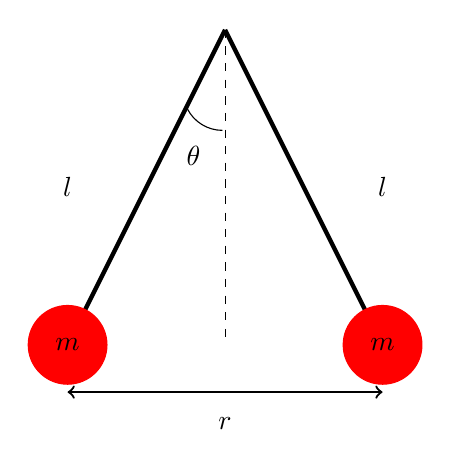
\begin{tikzpicture}
      \draw [ultra thick] (0,0) -- (2,4);
      \draw [ultra thick] (2,4) -- (4,0);
      \draw [dashed] (2,4) -- (2,0);
      \draw [red, fill] (0,0) circle [radius=0.5];
      \draw [red, fill] (4,0) circle [radius=0.5];
      \draw [thick, <->] (0,-0.6) -- (4,-0.6);
      \draw (1.52,3) arc [radius=0.5, start angle=206.6, end angle=270];
      \node at (0,2) {\(l\)};
      \node at (4,2) {\(l\)};
      \node at (0,0) {\(m\)};
      \node at (2,-1) {\(r\)};
      \node at (4,0) {\(m\)};
      \node at (1.6,2.4) {\(\theta\)};
    \end{tikzpicture}
    \caption{Pith balls on a string of length \(l\) with mass \(m\) and a distance \(r\) from each other.}
  \end{center}
\end{figure}

\subsection* {DATA}
Each combination of rod and material were used to charge the rod and apply it to the pith balls. The distance was then recorded for three trials. These trials are shown in Table 1. Tables 2 and 3 show the charge force, \(F_{\text{charge}}\), and charge magnitude, \(|q|\), for each rod/material pair. The mass of each pith ball was 0.04 grams per the lab manual (IIT, 3). The length of the string was not measured, but a value of 9.3 cm was used.

\begin {table}[H]
  \centering
  \begin {tabular}{| c | c | r | r | r | r |}
    \hline\hline
    & & \multicolumn {4}{| c |}{Rods} \\
    \hline
    & & Rubber & Nylon & Acrylic & Vinyl \\
    \hline
    \multirow {12}{*}{Material} & \multirow {3}{*}{Silk} & 0.0570 & 0.0080 & 0.0740 & 0.0250 \\
    & & 0.0550 & 0.0050 & 0.0660 & 0.0570 \\ 
    & & 0.0565 & 0.0070 & 0.0520 & 0.0660 \\
    \cline{2-6}
    & Average & 0.0562 & 0.00667 & 0.064 & 0.0493 \\ %66667 (LDR) %6667 (LDR) % %33333 (LDR)
    \cline{2-6}
    & \multirow {3}{*}{Plastic} & 0.0430 & 0.0070 & 0.0780 & 0.0640 \\
    & & 0.0300 & 0.0110 & 0.0640 & 0.0670 \\
    & & 0.0360 & 0.0090 & 0.0300 & 0.0640 \\
    \cline{2-6}
    & Average & 0.0363 & 0.009 & 0.0573 & 0.0650 \\ %33333 (LDR) % %33333 %
    \cline{2-6}
    & \multirow {3}{*}{Hair} & 0.0570 & 0.0620 & 0.0450 & 0.0710 \\
    & & 0.0600 & 0.0710 & 0.0650 & 0.0610 \\
    & & 0.0650 & 0.0660 & 0.0630 & 0.0660 \\
    \cline{2-6}
    & Average & 0.0607 & 0.0663 & 0.0577 & 0.0660 \\ %66667 (LDR) %33333 %66667 (LDR) %
    \cline{2-6}
    & \multirow {3}{*}{Wool} & 0.0480 & 0.0170 & 0.0340 & 0.0700 \\
    & & 0.0240 & 0.0060 & 0.0300 & 0.0730 \\
    & & 0.0300 & 0.0070 & 0.0560 & 0.0750 \\
    \cline{2-6}
    & Average & 0.0340 & 0.0100 & 0.0400 & 0.0727 \\ % % % %66667 (LDR)
    \cline{2-6}
    \hline\hline
  \end {tabular} \\
  \caption {Distance between pith balls in meters between different rods and materials.}
\end {table}

\begin {table}[H]
  \centering
  \begin {tabular}{| c | c | c | c | c | c | c | c | c | c |}
    \hline\hline
    & & \multicolumn {4}{| c |}{Rods} \\
    \hline
    & & \multicolumn {2}{| c |}{Rubber} & \multicolumn {2}{| c |}{Nylon} \\
    \hline
    & & \(F_{\text{charge}}\) N & \(|q|\) C & \(F_{\text{charge}}\) N & \(|q|\) C \\ 
    \hline
    \multirow {4}{*}{Material} & Silk & 0.000124 & 6.60 \(\times 10^{-9}\) & 0.0000141 & 2.63 \(\times 10^{-10}\) \\ %169358 %727543 (LDR) %592135 (LDR) %492357 %65347 (LDR) %568429 (LDR) %83345 (LDR) %002727
    \cline{2-6}
    & Plastic & 0.0000781 & 3.38 \(\times 10^{-9}\) & 0.0000190 & 4.13 \(\times 10^{-10}\) \\ %776033 (LDR) %413143 %899857 (LDR) %412471 %016292 %107479 %207576 %470485
    \cline{2-6}
    & Hair & 0.000135 & 7.44 \(\times 10^{-9}\) & 0.000150 & 8.55 \(\times 10^{-9}\) \\ %253239 %708455 (LDR) %638717 (LDR) %327732 %833041 (LDR) %26647 %778135 (LDR) %578913 (LDR)
    \cline{2-6}
    & Wool & 0.0000729 & 3.06 \(\times 10^{-9}\) & 0.0000211 & 4.84 \(\times 10^{-10}\) \\ %839413 (LDR) %966295 (LDR) %057941 %261111 %207909 %738668 (LDR) %368938 %984447 (LDR)
    \cline{2-6}
    \hline\hline
  \end {tabular} \\
  \caption {Force of charge and charge values for rubber and nylon}
\end {table}

\begin{table}[h!]
  \centering
  \begin{tabular}{| c | c | c | c | c | c |}
    \hline\hline
    & & \multicolumn {4}{| c |}{Rods} \\
    \hline
    & & \multicolumn {2}{| c |}{Acrylic} & \multicolumn {2}{| c |}{Vinyl} \\
    \hline
    & & \(F_{\text{charge}}\) N & \(|q|\) C & \(F_{\text{charge}}\) N & \(|q|\) C \\ 
    \hline
    \multirow {4}{*}{Material} & Silk & 0.000144 & 8.09 \(\times10^{-9}\) & 0.000108 & 5.40 \(\times 10^{-9}\) \\
    \cline{2-6}
    & Plastic & 0.000127 & 6.81 \(\times10^{-9}\) & 0.000146 & 8.28 \(\times 10^{-9}\) \\
    \cline{2-6}
    & Hair & 0.000128 & 6.87 \(\times10^{-9}\) & 0.000149 & 8.49 \(\times 10^{-9}\) \\
    \cline{2-6}
    & Wool & 0.0000863 & 3.92 \(\times10^{-9}\) & 0.000166 & 9.88 \(\times10^{-9}\) \\
    \hline\hline
  \end{tabular}
  \caption{Force of charge and charge values for acrylic and vinyl}
\end{table}

\subsection* {ANALYSIS OF DATA}
Figures 2 through 5 show the distance between the pith balls depending on the rod and material combination. Equation 9 from Supplementary Question 1 can be used to measure the force from Coulomb's Law. Figure 6 shows the force of the two charges using Equation 9 and the distance between the charges, while Figure 7 is a direct representation of Equation 13 and explores the distance between charges and the charge values themselves. \\

\noindent
Note: For comprehensibility, Figures 2 through 5 have been shown in centimeters.

\begin{figure}
  \centering
  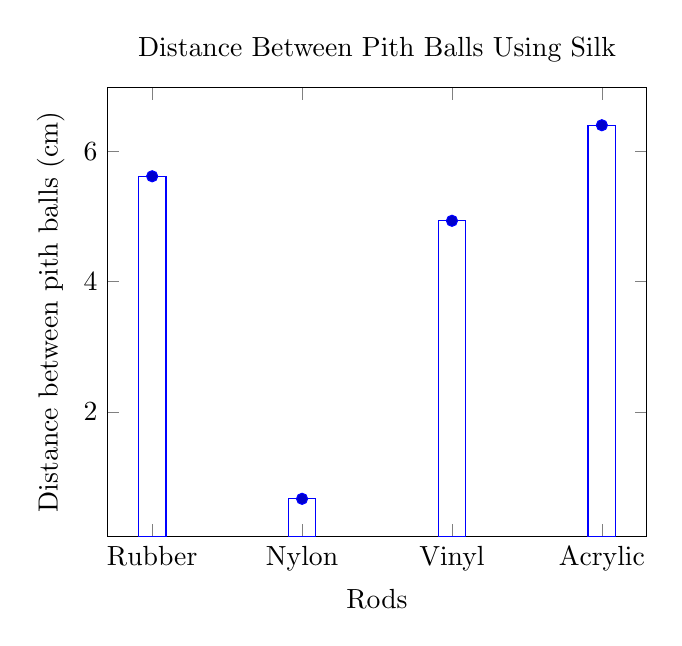
\begin{tikzpicture}
    \begin{axis}[
      title = {Distance Between Pith Balls Using Silk},
      symbolic x coords = {Rubber, Nylon, Vinyl, Acrylic},
      xtick = data,
      nodes near coords align={vertical},
      xlabel = {Rods},
      ylabel = {Distance between pith balls (cm)},
    ]
    \addplot+[ybar] plot coordinates
        {(Rubber,5.6166667) (Nylon, 0.6666667) (Vinyl,4.9333333) (Acrylic,6.4)};
    \end{axis}
  \end{tikzpicture}%
  \caption{}
\end{figure}

\begin{figure}[h!]
  \centering
  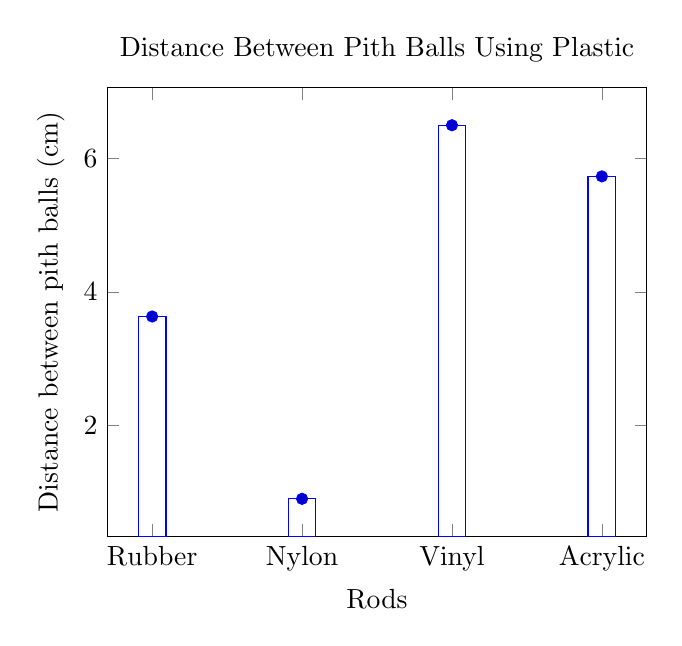
\begin{tikzpicture}
    \begin{axis}[
      title = {Distance Between Pith Balls Using Plastic},
      symbolic x coords = {Rubber, Nylon, Vinyl, Acrylic},
      xtick = data,
      nodes near coords align={vertical},
      xlabel = {Rods},
      ylabel = {Distance between pith balls (cm)},
    ]
    \addplot+[ybar] plot coordinates
        {(Rubber,3.6333333) (Nylon,0.9) (Vinyl,6.5) (Acrylic,5.7333333)};
    \end{axis}
  \end{tikzpicture}
  \caption{}
\end{figure}

\begin{figure}[h!]
  \centering
  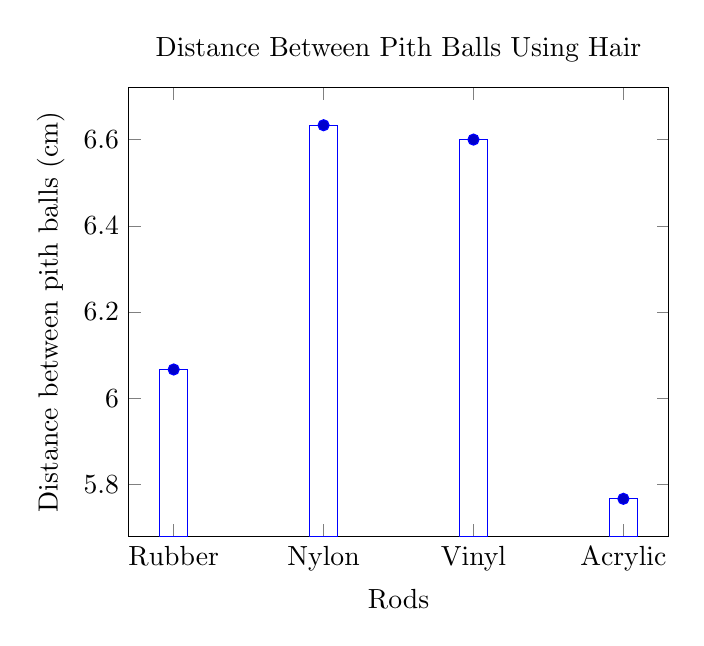
\begin{tikzpicture}
    \begin{axis}[
      title = {Distance Between Pith Balls Using Hair},
      symbolic x coords = {Rubber, Nylon, Vinyl, Acrylic},
      xtick = data,
      nodes near coords align={vertical},
      xlabel = {Rods},
      ylabel = {Distance between pith balls (cm)},
    ]
    \addplot+[ybar] plot coordinates
        {(Rubber,6.0666667) (Nylon,6.6333333) (Vinyl,6.6) (Acrylic,5.7666667)};
    \end{axis}
  \end{tikzpicture}
  \caption{}
\end{figure}

\begin{figure}[h!]
  \centering
  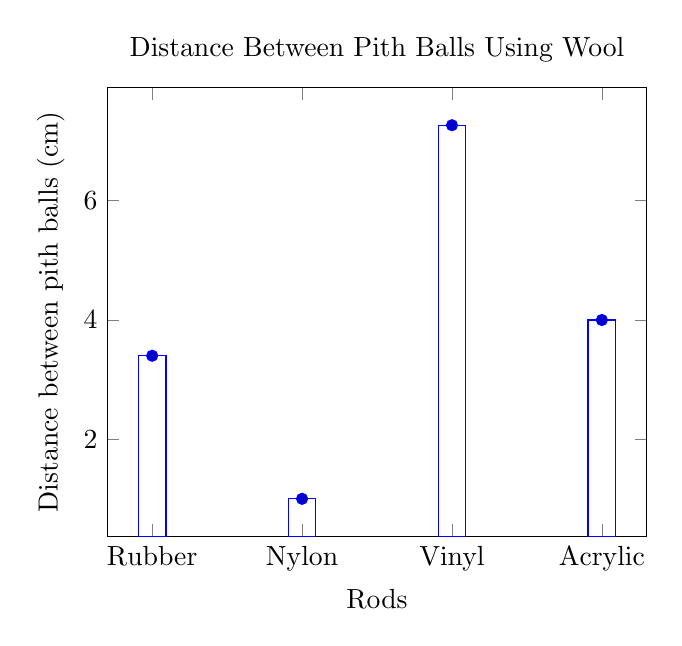
\begin{tikzpicture}
    \begin{axis}[
      title = {Distance Between Pith Balls Using Wool},
      symbolic x coords = {Rubber, Nylon, Vinyl, Acrylic},
      xtick = data,
      nodes near coords align={vertical},
      xlabel = {Rods},
      ylabel = {Distance between pith balls (cm)},
    ]
    \addplot+[ybar] plot coordinates
        {(Rubber,3.4) (Nylon,1) (Vinyl,7.2666667) (Acrylic,4)};
    \end{axis}
  \end{tikzpicture}
  \caption{}
\end{figure}

\pgfplotstableread{
X Y
0.056166667 0.000124169358 
0.006666667 0.0000140592135
0.064       0.00014365347
0.049333333 0.00010783345
0.036333333 0.0000780776033
0.009       0.0000189899857
0.057333333 0.000127016292
0.065       0.000146207576
0.060666667 0.000135253239
0.066333333 0.000149638717
0.057666667 0.000127833041
0.066       0.000148778135
0.034       0.0000728839413
0.01        0.0000211057941
0.04        0.0000863207909
0.072666667 0.000166368938
}\distanceAndForce

\begin {figure}
  \centering
  \begin{tikzpicture}
    \begin{axis}[
      title = {Distance Between Charges and Force of Charge},
      xlabel = {\(r\) (m)},
      ylabel = {\(F_{\text{charge}}\) (N)},
      ]
      \addplot [only marks, mark = *] table {\distanceAndForce};
      \addplot [thick, red] table[
        y={create col/linear regression={y=Y}}
      ]
      {\distanceAndForce};
    \end{axis}
  \end{tikzpicture}
  \caption {}
\end {figure}

\pgfplotstableread{
X Y
0.056166667 0.00000000659727543
0.006666667 0.000000000263492357
0.064       0.00000000808568429
0.049333333 0.00000000540002727

0.036333333 0.00000000338413143
0.009       0.000000000413412471
0.057333333 0.00000000681107479
0.065       0.00000000828470485

0.060666667 0.00000000743708455
0.066333333 0.000000000484261111
0.057666667 0.00000000391738668
0.066       0.00000000987984447

0.034       0.00000000305966295
0.01        0.000000000484261111
0.04        0.00000000391738668
0.072666667 0.00000000987984447
}\distanceAndCharge

\begin {figure}
  \centering
  \begin{tikzpicture}
    \begin{axis}[
      title = {Distance Between Charges and Charge Values},
      xlabel = {\(r\) (m)},
      ylabel = {\(q\) (C)},
      ]
      \addplot [only marks, mark = *] table {\distanceAndCharge};
      \addplot [thick, red] table[
        y={create col/linear regression={y=Y}}
      ]
      {\distanceAndCharge};
    \end{axis}
  \end{tikzpicture}
  \caption {}
\end {figure}

\subsection* {DISCUSSION OF RESULTS}
Figures 2 through 5 can be compared to what was expected for each rod/material combination. For instance, in Figure 2, it was expected that the acrylic rod would show the greatest distance between pith balls followed by vinyl, with nylon and rubber being equal. However, Figure 2 shows that while acrylic discharged the most, nylon and rubber did not behave as expected. \\\\
For plastic, it was expected that acrylic would show the greatest distance, followed by nylon, vinyl, and then rubber. The lowest, as shown in Figure 3, was nylon, which does not match expectations. \\\\
For hair, the expectation was for vinyl to discharge the greatest, followed by rubber, and equally, acrylic and nylon. However, nylon again disrupts expectations by having the greatest distance between the pith balls. Acrylic and rubber seem to follow expectations. \\\\
And lastly, for wool, vinyl was expected to show the greatest distance, followed by rubber, acrylic, and nylon. Figure 5 shows that these expectations were mostly met, with acrylic slightly exceeding the distance expected. \\

\subsection* {FURTHER STUDY}

\subsection* {SUPPLEMENTARY QUESTIONS}
1. How does the potential vary with distance on your plots?
The potential will 
2. Calculate the electric field strength at a few places with different characteristics using Eq. 2. Do your results agree with the idea that electric field line density is proportional electric field strength? Sketch neatly and clearly an appropriate amount of lines on your grid paper. You may want to use a different color.
3. Consider the following situation: An object with charge qo= 1.5μ C and mass 0.7 g starts from rest at the +6V equipotential line. Calculate its change in potential energy and speed when it reaches the +2V line.

\subsection* {REFERENCES}
Boston University. (n.d.). Electric charge and Coulomb's law. Retrieved February 5, 2020, from https://physics.bu.edu/~duffy/py106/Charge.html \\\\
Gladding, G., Selen, M. A., \& Stelzer, T. (2012). Electricity and Magnetism. New York: W.H. Freeman. \\\\
Illinois Institute of Technology. (n.d.). Experiment 1: Coulomb's Law. PDF. Chicago.
\end {document}
